\documentclass[tikz,border=3pt]{standalone}
\usepackage[T1]{fontenc}
\usepackage{lmodern}
\usepackage{amsmath}
\usetikzlibrary{arrows.meta,positioning}
\begin{document}
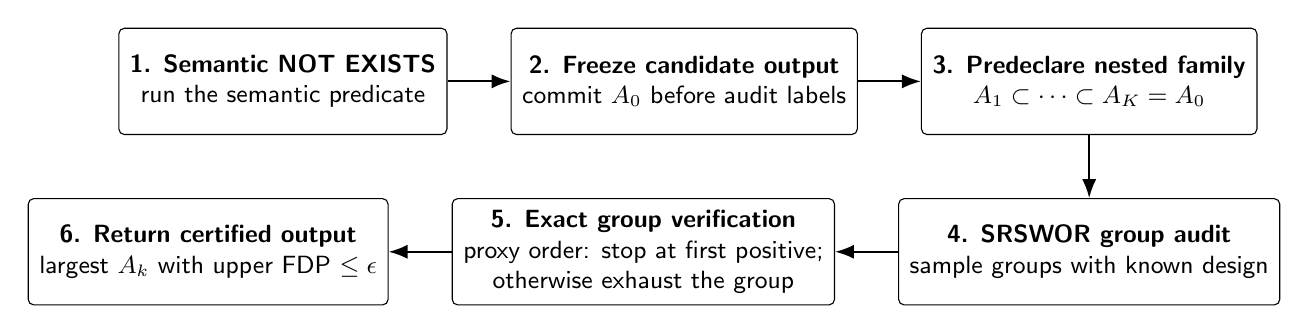
\begin{tikzpicture}[
  font=\sffamily\small,
  node distance=8mm and 8mm,
  certbox/.style={draw, rounded corners=2pt, align=center, minimum width=4.05cm, minimum height=1.35cm, inner sep=4pt},
  flow/.style={-{Latex[length=2.4mm]}, line width=.75pt}
]
\node[certbox] (q) {\textbf{1. Semantic NOT EXISTS}\\run the semantic predicate};
\node[certbox, right=of q] (freeze) {\textbf{2. Freeze candidate output}\\commit $A_0$ before audit labels};
\node[certbox, right=of freeze] (nested) {\textbf{3. Predeclare nested family}\\$A_1\subset\cdots\subset A_K=A_0$};

\node[certbox, below=of nested] (sample) {\textbf{4. SRSWOR group audit}\\sample groups with known design};
\node[certbox, left=of sample] (verify) {\textbf{5. Exact group verification}\\proxy order: stop at first positive;\\otherwise exhaust the group};
\node[certbox, left=of verify] (return) {\textbf{6. Return certified output}\\largest $A_k$ with upper FDP $\leq\epsilon$};

\draw[flow] (q) -- (freeze);
\draw[flow] (freeze) -- (nested);
\draw[flow] (nested) -- (sample);
\draw[flow] (sample) -- (verify);
\draw[flow] (verify) -- (return);
\end{tikzpicture}
\end{document}
